%%%%%%%%%%%%%%%%%%%%
% Copyright and authorship: Fernando Oleo Blanco.
%
% Thanks to all the people that helped me get to where I am.
% Free use, just acknowledge the authors.
%%%%%%%%%%%%%%%%%%%%

%%%%%%%%%%%%%%%%%%%%
% IMPORTANT
% THIS DOCUMENT REQUIRES LuaLaTeX OR XeLaTeX AS THE PROCESSING ENGINE
% SOME "SPECIAL" VARIABLES HAVE BEEN SET AT THE BOTTOM OF THE FILE TO HELP
% IT SHOULD WORK AUTOMATICALLY WITH TeXstudio AND Emacs
%%%%%%%%%%%%%%%%%%%%

%%%
% Important. The packages and some extra functionallity is found in the loaded-thesis.sty file!
% Read it to learn more about what you can do with LaTeX and how things are configured.
%%%

% General document definition. In order to have the text completely centered, do not use the twoside option; however, twoside is recommended for printing.
\documentclass[12pt, a4paper, twoside]{book}

% For general information and help about LaTeX, refer to https://www.overleaf.com/learn

%%% Packages
% Please, read the "loaded-thesis.sty" document to see what is actually loaded and how to use it. Some configuration options for a set of packages is also present there. Change those if you need it.
\usepackage{loaded-thesis}

%% Language configuration
\setdefaultlanguage[variant=british]{english} % Adds localization support to XeTeX and LuaLaTeX. Replaces babel!
% Select your prefered language. Example: \usepackage[activeacute, spanish]{polyglossia}
% IMPORTANT: if you compile the document with one language (say english) and then change it to another, the automatically generated files in the directory need to be deleted! Especially the .aux file!


%% Bibliography configuration

\usepackage[backend=biber,
			style=numeric,
			sorting=none]{biblatex}
			% Citation configuration. We use biblatex, which is more
			% complex, but as customizable as it gets.
			% Please, modify this to your liking.
			% IMPORTANT: this requires biber to be installed and run every time
			% you change the .bib file! To make it easier, if you are using TeXStudio, do the following:
			% 1. Go to options. 2. Select the Build menu. 3 In standard bibliography, change bibtex to biber. 4. Profit
			% These changes will allow the editor to detect any changes and "recompile" the files if needed.
			% For other editors see: https://tex.stackexchange.com/questions/154751/biblatex-with-biber-configuring-my-editor-to-avoid-undefined-citations
			% See link for a quick introduction: https://tex.stackexchange.com/questions/26516/how-to-use-biber/34136
			% If you are having issues with the bibliography, please, search for how to install and run biber!

			% Specialised packages. Please, read their documentation as they provide a lot of functionallity.

% Bibliography resource
\addbibresource{main.bib} % Read bibliography entries/database

\renewcommand*{\nameyeardelim}{\addcomma\addspace} % To add a coma after et al. -> et al.,

%%% Acronyms and glossary

%% Force processing of glossaries
\makeglossaries

% Read the documentation of glossaries and glossaries-extra. They are incredibly powerful,
% but may require some fiddling to get things exactly how you may want them!

%% Acronyms
% The acronyms definitions are found in the acronym.tex file.
% Modify that file accordingly
\loadglsentries[\acronymtype]{acronyms.tex}
% Set the short-long style. It prints the long version the first time an acronym is used
\setabbreviationstyle[acronym]{long-short}

%% Glossary terms
\loadglsentries{glossaries.tex}

%%% Font configuration

% Change the mono font in order to support more Unicode characters
\setmonofont{DejaVu Sans Mono}[Scale=MatchLowercase]

% Link colour setup. If you want colours, set "colorlinks" to "true"
\hypersetup{
	colorlinks = false,
	citecolor = red,
	urlcolor = blue,
} % Change this options to your liking

%%% Custom commands

% Add abstract environment to book style
\newenvironment{abstract}%
{\cleardoublepage \null \vfill \begin{center}%
		\bfseries \abstractname \end{center}}%
{\vfill\null}

% Hide environments

% Hide plots to speed up processing by uncommenting the following line
\newif\ifhidepgfplots
%\hidepgfplotstrue % Comment to hide plots
\ifhidepgfplots
 \usepackage{environ}
 \NewEnviron{hide}{}
 \let\tikzpicture\hide
 \let\endtikzpicture\endhide
\fi

\newfloat{genericfloat}{tbhp}{lop} % Added due to bad interaction between dpfloat and algorithm2e

%%% DOCUMENT

\begin{document}
	% Include the cover. Modify to your liking
	\pagestyle{empty} % Suppress the "fancy" hearders in the front matter

% Change the page geometry to have a little bit more space
%\newgeometry{left=2.5cm,bottom=3cm,right=2.5cm}

% Begin title page
\begin{center}
	% Logo
	\begin{figure}
		\centering
		
\includegraphics[width=0.3\linewidth]{LogoUniversidadBN}
	\end{figure}
	% University degree
	\Large Degree in Industrial Technologies \\ % Modify accordingly
	\vspace*{2.5em} % This just adds some vertical spacing
	% Type of work
	Bachelor's or Master's final project \\ % Modify accordingly
	\vspace*{1em}
	% Title of your work
	This is the title of your project
	\\ \large
	\vspace*{3em}
	Author \\
	% Author's name
	Author's Name \\
	\vspace*{1em}
	% Add supervisors or directors
	Supervised by \\ Prof. Dr. Mc Great$^a$ \\ Prof. Dr. Mc Amazing$^b$ \\
	$^a\,${\footnotesize Institute of Greatness} \\ $^b\,${\footnotesize Amazing University}
	% Uncoment this line if you would like to add a signature space
	% {\vfill \vspace*{3em}{Author's signature:\hrulefill \hfill} \hfill \\ \vspace*{4em}Supervisors' signatures:\hrulefill \hfill}
	\vfill
	München 2022 % Modify accordingly
\end{center}

% Restore the geometry that was defined
%\restoregeometry
% Next page should open on the right
\cleardoublepage

	\frontmatter % First few pages

	% Coment this block if you don't want a dedication and prelude information page
	% Thanks and other information page
	{\centering Thank yous\\}
	\vfill % Fill the page with whitespace (this is just for aesthetic reasons)
	And other important information

	\cleardoublepage

	% Write your abstract
	\begin{abstract}
		Abstract content
	\end{abstract}

	\cleardoublepage % New page starts on the right hand side

	\tableofcontents % Create the index
	\listoffigures % Create index of figures
	\listoftables % Create index of tables
	\lstlistoflistings % Create index for code sections
	\listofalgorithms % Create index for algorithms
	\printglossary[title=List of Symbols, style=longheader, nonumberlist] \label{glossaries} % Create glossary enty
	\setlength{\glspagelistwidth}{0.2\linewidth} % Add a bit more width to the "Page List" column
	\printglossary[type=\acronymtype, style=long3col-booktabs] % Create acronym entry

	\cleardoublepage % Open on right hand page (odd numbered)

	% Main body of the work
	\mainmatter

	% Activate customized headers
	\pagestyle{fancy}

	% Include the different chapters, documents etc
	\chapter{An overview of \LaTeX}

In this section, a few basic tools will be presented. In following sections more advance functionality and complex tools will be showcased. \textbf{Use this as examples and to your advantage!}

\textsc{\color{red}Important:} this template uses Lua\LaTeX, a modern \LaTeX\ engine. You should setup your editor to use Lua\LaTeX, otherwise it will not be able to generate the document. Overleaf, for example, does not change the \LaTeX\ engine automatically, so you have to do it yourself (it is very easy!).

\textsc{\color{red}Important:} read the documentation of the pacakges that you will use! Also, read general documentation about \LaTeX! While the following guide below explains some of the most basic and cooler topics of \LaTeX, the explanations are swallow. I do not cover details nor issues that may appear and how to fix them. Some really good resources are:
\begin{itemize}
	\item \href{https://en.wikibooks.org/wiki/LaTeX}{\LaTeX's Wikibook}
	\item \href{https://www.overleaf.com/learn}{Overleaf's \LaTeX\ resources}
	\item \href{https://www.ctan.org/tex-archive/info/lshort/english/}{The not so short introduction to \LaTeX} book
	\item {\color{red} The packages manuals!}
	\item Any searh engine.
\end{itemize}

\section{Basics of \LaTeX}

\subsection{Text styles}

The following table showcases some of the more common text styles in \LaTeX.

\begin{table}[h]
	\centering
	\begin{tabular}{lcc}
	  \toprule
	  Style & Code & Ouput \\
	  \midrule
	  Quotes & \verb|``Quotes''| & ``Quotes'' \\
	  Boldface & \verb|\textbf{Boldface}| & \textbf{Boldface} \\
	  Italics & \verb|\textit{Italics}| & \textit{Italics} \\
	  Emphasis & \verb|\emph{Emphasis}| & \emph{Emphasis} \\
	  Underline & \verb|\underline{Underline}| & \underline{Underline} \\
	  Typewriter & \verb|\texttt{Typewriter}| & \texttt{Typewriter} \\
	  Small caps & \verb|\textsc{small caps}| & \textsc{small caps} \\
	  Mathematical & \verb|$Mathematical^{\pi\cdot i}$| & $Mathematical^{\pi\cdot i}$ \\
	  \LaTeX\ Comments & \verb|% Some text| & % Some text
	  \\
	  \bottomrule
	\end{tabular}
	\caption{Text styles in \LaTeX.}
	\label{fig:textstyles}
\end{table}

\subsection{Structure of a \LaTeX\ document}

For this template, which is based in the \texttt{book} class, we have the following major sections:

\begin{enumerate}
	\item \verb|\part{}|: Parts are fully self-contained portions of information. They leave a full blank page with only the title of the part. \textbf{This is not used and not recommended!}
	\item \verb|\chapter{}|: Your normal chapters, as you can see above. We are in the ``\emph{An overview of \LaTeX }.''
	\item \verb|\section{}|: Normal sections for a chapter. We are in ``\emph{Basics of \LaTeX}.''
	\item \verb|\subsection{}|: Subsections. We are in ``\emph{Structure of a \LaTeX\ document}.''
	\item \verb|\subsubsection{}|: Subsubsections. This level tends to be quite deep and will most likely not appear in the index unless we include \verb|\setcounter{secnumdepth}{3}| in the preamble\footnote{The preamble is the part before \texttt{\textbackslash begin\{document\}}, basically, the setup section.}.
	\item \verb|\paragraph{}|: One step deeper. By default paragraphs are not numbered.
\end{enumerate}

You jus have to write what you want between the \verb|{}| for each command, and \LaTeX\ does the rest. It typsets the titles/sections, it adds them to the table of contents and numbers them consistently!

\subsection{Mathematical notation}

\LaTeX\ provides several way to include symbols and write maths. The most basic way is to include mathematical notation or symbols into the text. This is known as \emph{inline} and can be done with \verb|$...$|. Whatever is between the \$ symbols, is typeset in mathematical notation. This is an example: $2 = \frac{4}{2}$. This is produced using \verb|$2 = \frac{4}{2}$|.

Another method is to write mathematical formulas in \emph{display} mode, which is separated from the text. This can be done by wrapping the text in \verb|\[...\]|. \textbf{This is not recommended} as the next method is better. Here is an example:

\[
	2 = \frac{4}{2}
\]

Normally, the best way is to use mathematical environments. This environments will provide more functionality and generally number the equations and allows them to be labelled. Here are a few examples:

\begin{equation} \label{eq:simpleeq}
	2 = \frac{4}{2}
\end{equation}

The equation above, \cref{eq:simpleeq}, is produced by writing:

\begin{lstlisting}[language={[LaTeX]TeX}]
\begin{equation} \label{eq:simpleeq}
	2 = \frac{4}{2}
\end{equation}
\end{lstlisting}

Lets showcase some more environments that help us write beautiful formulas! The \verb|\begin{array}| environment helps us write vertically aligned formulas!

\begin{equation} \label{eq:abaqus-exponential-decay}
f(t) = \left\{
	\begin{array}{lcc}
		A_0 + A\cdot e^{-\dfrac{t - t_0}{t_d}} & for & t \geq t_0 \\
		A_0 & for & t < t_0
	\end{array}
	\right.
\end{equation}

\begin{lstlisting}[language={[LaTeX]TeX}]
\begin{equation} \label{eq:abaqus-exponential-decay}
	f(t) = \left\{
	\begin{array}{lcc}
		A_0 + A\cdot e^{-\dfrac{t - t_0}{t_d}} & for & t \geq t_0 \\
		A_0 & for & t < t_0
	\end{array}
	\right.
\end{equation}
\end{lstlisting}


The \verb|\begin{aling}| environment may be easier to use, but it has a few quirks. Read the documentation\footnote{\url{http://tug.ctan.org/info/short-math-guide/short-math-guide.pdf}} for more information.

\begin{align}
	a_{11}& =b_{11}&
	a_{12}& =b_{12}\\
	a_{21}& =b_{21}&
	a_{22}& =b_{22}+c_{22}
\end{align}

\begin{lstlisting}[language={[LaTeX]TeX}]
\begin{align}
	a_{11}& =b_{11}&
	a_{12}& =b_{12}\\
	a_{21}& =b_{21}&
	a_{22}& =b_{22}+c_{22}
\end{align}
\end{lstlisting}

The \verb|\begin{subequations}| allows us to have several formulas numbered into the same reference. As shown in \cref{eq:symmetry-bc}, with the first entry being \cref{eq:x-symmetry-bc}.

\begin{subequations} \label{eq:symmetry-bc}
	\begin{equation} \label{eq:x-symmetry-bc}
		\text{\texttt{XSYMM}} \equiv U1 = UR2 = UR3 = 0
	\end{equation}
	\begin{equation}
		\text{\texttt{ZSYMM}} \equiv U3 = UR1 = UR2 = 0
	\end{equation}
\end{subequations}

\begin{lstlisting}[language={[LaTeX]TeX}]
\begin{subequations} \label{eq:symmetry-bc}
	\begin{equation} \label{eq:x-symmetry-bc}
		\text{\texttt{XSYMM}} \equiv U1 = UR2 = UR3 = 0
	\end{equation}
	\begin{equation}
		\text{\texttt{ZSYMM}} \equiv U3 = UR1 = UR2 = 0
	\end{equation}
\end{subequations}
\end{lstlisting}

\subsection{References}

One of the strongest points of \LaTeX\ is its wonderful and powerful referencing system. We can reference whatever we want by putting on a ``tag'' with the command \verb|\label{xxx}|. Wherever the \verb|\label| is, it will refer to it. You can see some examples above where we refered to a few equations by their labels, which are inside the \verb|\begin{equation}| environment. This way, \LaTeX\ knows automatically what type of thing they are referring.

The different types of references are shown in \cref{tab:reference-systems}.

\begin{table}[h]
	\centering
	\begin{tabular}{lcc}
	  \toprule
	  Package & Command & Result \\
	  \midrule
	  \LaTeX & \verb|\ref{eq:simpleeq}| & \ref{eq:simpleeq} \\
	  & \verb|\pageref{eq:simpleeq}| & \pageref{eq:simpleeq} \\
	  \cmidrule{2-3}
	  \texttt{hyperref} & \verb|\autoref{eq:simpleeq}| & \autoref{eq:simpleeq} \\
			  & \verb|\autoref{fig:textstyles}| & \autoref{fig:textstyles} \\
			  & \verb|\autopageref{eq:simpleeq}| & \autopageref{eq:simpleeq} \\
	  \cmidrule{2-3}
	  \texttt{cleveref} & \verb|\cref{eq:simpleeq}| & \cref{eq:simpleeq} \\
			  & \verb|\Cref{eq:simpleeq}| & \Cref{eq:simpleeq} \\
	  & \verb|\cpageref{eq:simpleeq}| & \cpageref{eq:simpleeq} \\
			  & \verb|\cref{eq:simpleeq,eq:symmetry-bc}| & \cref{eq:simpleeq,eq:symmetry-bc} \\
			  & \verb|\crefrange{eq:simpleeq}| & \multirow{2}{*}{\crefrange{eq:simpleeq}{eq:symmetry-bc}}\\
	  & \verb|{eq:symmetry-bc}| & \\
	  \bottomrule
	\end{tabular}
	\caption[Different reference mechanisms.]{Different reference mechanisms. \textbf{The author recommends \texttt{cleveref}!}. It is included in this template.}
	\label{tab:reference-systems}
\end{table}

\subsection{Bibliography}

Bibliography management is another strong point of \LaTeX! We just need to add bibliographic entries to the bibliography database, which for this template it is the \texttt{main.bib} file. Here is what such an entry can look like:

\begin{lstlisting}[language={[LaTeX]TeX}]
@book{lovecraft2016el,
	author = {Lovecraft, H. P.},
	title = {El clérigo malvado y otros relatos},
	publisher = {Alianza Editorial},
	year = {2016},
	address = {Madrid},
	isbn = {9788491042105}
}
\end{lstlisting}

In order to cite the entry we just have to use \verb|\cite{}| with the entry's identifier, like so \verb|\cite{lovecraft2016el}| \cite{lovecraft2016el}. We can also have multiple cites in the same command, \cite{lovecraft2016el,norton_creep} (\verb|\cite{lovecraft2016el,norton_creep}|). It is that simple! They get automatically printed in the bibliography section.

\textsc{\color{red}Important:} this template uses \texttt{biblatex} as the management system, which is a powerful, flexible and modern tool. Therefore, you will need to run the \texttt{biber} command to build the bibliography after the first compilation of your document; then you will have to recompile after \texttt{biber} has run. Most editors do this by default.

You can also use third-party tools like Zotero\footnote{\url{https://www.zotero.org/}} to manage your \verb|.bib| database. Most bibliography management tools are capable of dealing with \verb|.bib| entries!

\subsection{Tables, images and floating environments}

Probably, the part of \LaTeX\ that causes the most confusion among new users, are the so called \emph{floating envrionments}. \textbf{Tables, images, algorithms, etc are floating envrionments}. This means that \textbf{\LaTeX\ can position them where it sees fit, not where they are written by the user.} In reality, \LaTeX\ is trying to optimise your document's layout and leave as little empty space as possible.

Sooo... How do we solve \LaTeX\ moving our floating environments? Here are a few solutions:

\begin{itemize}
	\item We don't solve it. \LaTeX\ referencing tools allow us to easily point the reader to the table, image, etc. Therefore, it is not that problematic that the \emph{floats} may not be where we put them!
	\item We can ask \LaTeX\ to try to place the image where it appears in our document. This is done with the \emph{``here''} \verb|[h]| placement modifier, more on placement modifiers later. \textbf{This is not a definitive solution.} This will just tell \LaTeX\ to try hard to do what we are asking. There is the \verb|[h!]| modifier, which is even stronger.
	\item \textbf{A really good solution is to use} \verb|\FloatBarrier|. It comes from the \verb|placeins| package, included in this template. \verb|\FloatBarrier| forces \LaTeX\ to put all floating environment that have already appeared before the position where \verb|\FloatBarrier| appears. This is very useful to force \LaTeX\ to put all floats before another section that may not be related to the topic of those floats. Here is an example:

\begin{lstlisting}[language={[LaTeX]TeX}]
\section{Some topic}

\begin{figure}
	XXX
\end{figure}

\begin{table}
	XXX
\end{table}

\FloatBarrier % All previous floats will appear before this point.

\section{Some unrelated topic}
XXX
\end{lstlisting}
	\item We can use the placement modifier \verb|[H]| to force the float to appear \emph{HERE}. This is provided by the \verb|float| package. However, \textbf{this solution is not recommended!} It can lead to some wierd and nasty document layouts!
\end{itemize}

Now, how do we actually include figures, tables, etc? They all follow the same structure, here are some examples:

\begin{description}
		\item[Figures] are declared in the \verb|figure| environment (\emph{\textsc{shock!}}). You can see the image rendered in \cref{fig:monoblock-overview-mesh}.

\begin{lstlisting}[language={[LaTeX]TeX}]
\begin{figure}
	\centering % Center image horizontally
	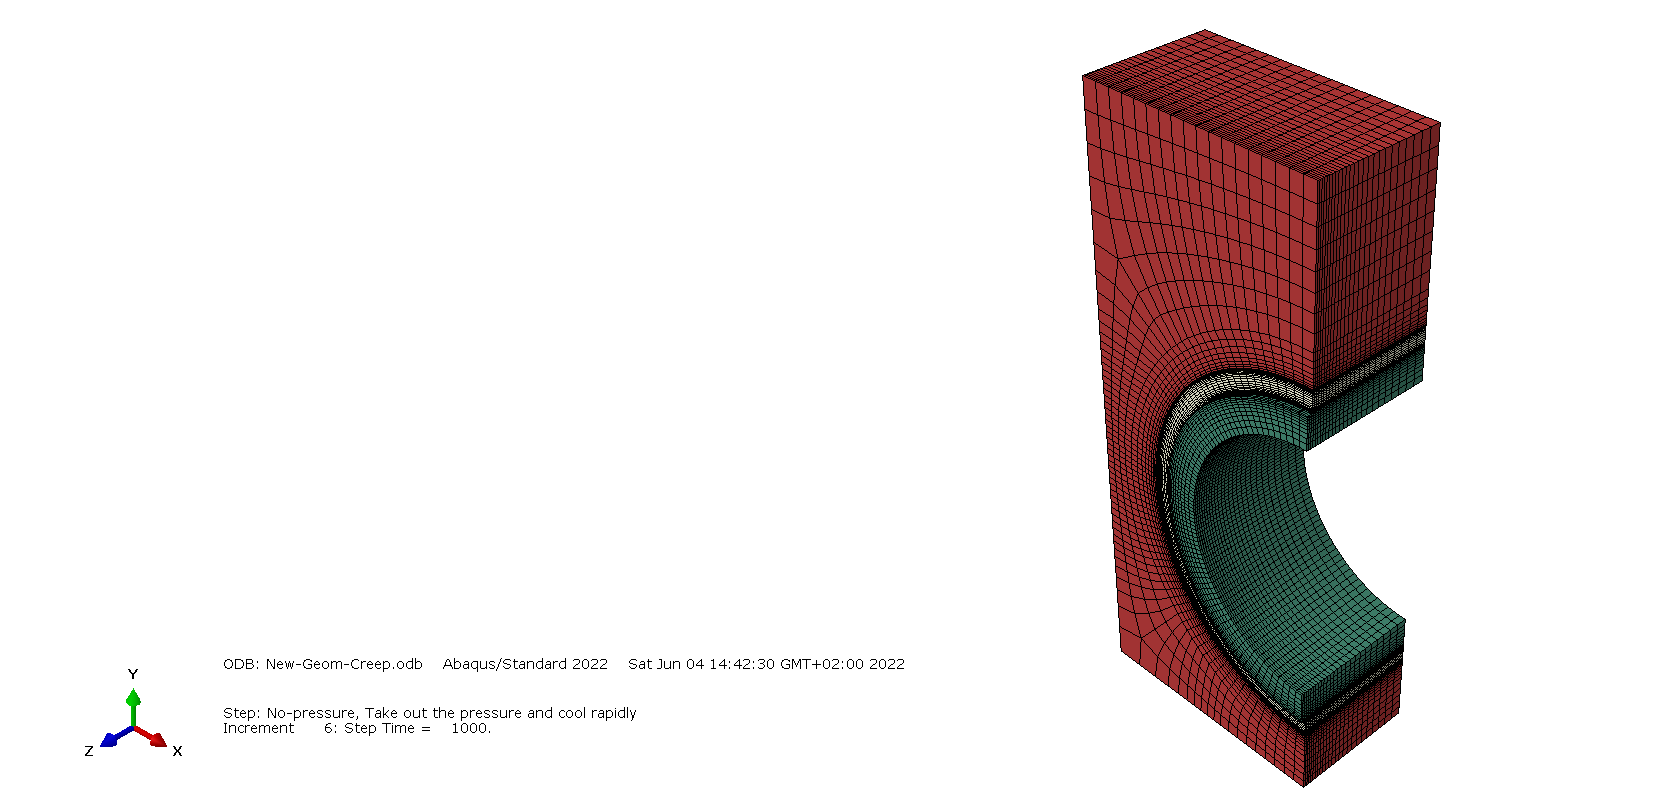
\includegraphics[keepaspectratio, trim = 1050 12 150 30, clip, width=0.5\linewidth, height=0.3\textheight]{Images/monoblock-material-overview-mesh.png}
	\caption[Overview of \glsentryname{FEM} mesh used for the final analysis.]{Overview of \glsxtrshort{FEM} mesh used for the final analysis.}
	\label{fig:monoblock-overview-mesh}
\end{figure}
\end{lstlisting}
	The key here is \verb|\includegraphics|, it is what loads the graphics and allows us to set its properties. The above example is rather complex, most times you do not need these many options. Nonetheless, here is what they do:
	\begin{description}
			\item[\texttt{keepaspectratio}] Keeps the size ratio of the image. Very useful if you set \verb|height| and \verb|width| at the same time.
			\item[\texttt{trim}] It allows us to trim/cut the image. It cuts X amount of pixels from the \texttt{left, bottom, right, top}. This is useful if your image is too large and you only care about a small portion of it.
			\item[\texttt{clip}] Only show the trimmed image.
			\item[\texttt{width} and \texttt{height}] Sets the maximum size with respect to the width and height. We use \verb|\linewidth| and \verb|\textheight| to limit the size of the image in the page by using the page's natural lengths.
	\end{description}

	Then we have \verb|\caption|, which is what adds the text to the image. We use \verb|\caption[]| here, to modify the text that will appear in the ``List of Figures'', as I do not want my acronym \texttt{FEM} to be linked there, and therefore I use \verb|\glsentryname| to control that. But more about acronyms and glossaries in \cref{sec:glossaries}
	Finally, we have \verb|\label{}| is is what allows us to give an identifier to our image so that we can reference it.
		\item[Tables] are fairly easy to do once we get used to their nature. It uses the \verb|table| floating environment with another environment that allows us to type tabulated data. A basic example is given below and shown in \cref{tab:example-table}.
\begin{lstlisting}[language={[LaTeX]TeX}]
\begin{table}
	\centering % To center the table
	\begin{tabular}{lcr}
	  \toprule
	  Heading 1 & Heading 2 & Heading 3 \\
	  \midrule
	  Left aligned & Center aligned & Right aligned \\
	  \cmidrule{2-3} % Example of a controled rule
	  Some info & Some info & Some info \\
	  \bottomrule
	\end{tabular}
	\caption{Example of a table.}
	\label{tab:example-table}
\end{table}
\end{lstlisting}
	\textsc{\color{red}Important:} the \texttt{\&} symbol is used as a column separator in all alignment environments!

	The column alingment options for the tabular environment can be \texttt{l, c, r, m{}} or \texttt{p{}} among others. They refer to left, center, right alignment and the \texttt{m{}} and \texttt{p{}} refer to a limited size column whose vertical alignment is either centered or natural. You could use them as \verb|m{0.3\linewidth}| for example. If you want to aling the text horizontally with \texttt{m} or \texttt{p} you would write \verb|>{\centering\arraybackslash}m{0.3\linewidth}|. You can change the \verb|\centering| for a \verb|\raggedright| for a right aligned column. But this is getting too advance!
	One final bit of knowledge about very long tables and dynamicly sized columns. This template includes the package \texttt{xltabular}, which includes the well-known \verb|tabularx| environment and merges it with the \verb|longtable| environment (for tables that can span more than one page) generating its own \verb|xltabular| envrionment. Please red the documentation of the \texttt{tabularx}, \verb|longtable| and \verb|xltabular| if you need to build complex tables!

	Also, \textbf{there are online tools to help you generate \LaTeX\ tables from Excel sheets}. One such example (which I am not very familiar with nor endorse) is \href{https://tableconvert.com/excel-to-latex}{Tableconvert}.

	Finally, if you have \texttt{.csv} files or similar and you want to print them in your \LaTeX\ document, you can see \cref{sec:pgfplotstable}, which shows how \cref{tab:automatic-reading-csv} was automatically generated using \verb|pgfplotstable|.
\end{description}

\begin{figure}[h]
	\centering % Center image horizontally
	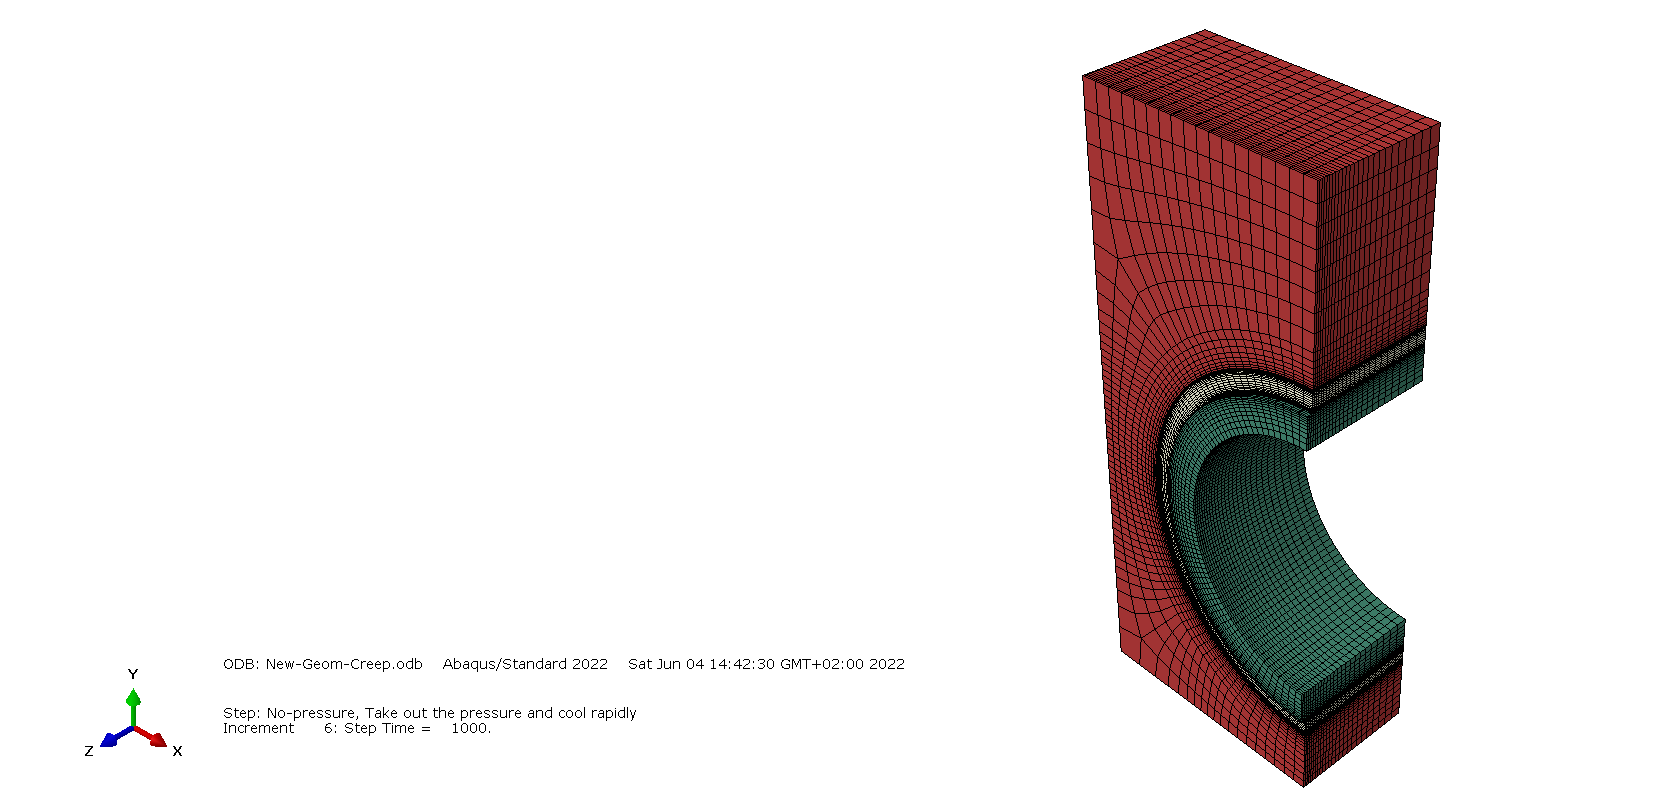
\includegraphics[keepaspectratio, trim = 1050 12 150 30, clip, width=0.5\linewidth, height=0.3\textheight]{Images/monoblock-material-overview-mesh.png}
	\caption[Overview of \glsentryname{FEM} mesh used for the final analysis.]{Overview of \glsxtrshort{FEM} mesh used for the final analysis.}
	\label{fig:monoblock-overview-mesh}
\end{figure}

\begin{table}[h]
	\centering % To center the table
	\begin{tabular}{lcr}
	  \toprule
	  Heading 1 & Heading 2 & Heading 3 \\
	  \midrule
	  Left aligned & Center aligned & Right aligned \\
	  \cmidrule{2-3} % Example of a controled rule
	  Some info & Some info & Some info \\
	  \bottomrule
	\end{tabular}
	\caption{Example of a table.}
	\label{tab:example-table}
\end{table}

\section{Glossaries}\label{sec:glossaries}

Creating glossaries in \LaTeX\ is surprisingly easy. However, it does require a bit of understanding.

For this template, the entries for the glossaries and acronyms (which are just a different type of glossary) are loaded from the \texttt{glossaries.tex} and \texttt{acronyms.tex} files. This is just to keep things organised. So, lets define some entries for our glossary and acronym list.

For glossary entries we use the \verb|\newglossaryentry{}{...}| command. Here is an example:

\begin{lstlisting}[language={[LaTeX]TeX}]
\newglossaryentry{identifier}
{
	name={name}, % Mandatory, what gets printed
	description={description of the entry}, % Mandatory, description that appears in the glossary index
	plural={plural-name}, % Optional, in case the plural is more complex
	sort={alphanumeric entry}, % Optional, how should the entry be sorted
	symbol={\ensuremath{associated symbol}}, % Optional, prints the symbol of the entry with \glssymbol{identifier}
}
\end{lstlisting}

For acronyms, we could use the code above, but there is a simpler and more direct way of doing it with \verb|\newabbreviation{}{}{}|. Here is how it works:

\begin{lstlisting}[language={[LaTeX]TeX}]
\newabbreviation{Identifier}{ACRONYM}{Description Of Acronym}
\end{lstlisting}

\verb|\newabbreviation[]| supports a long set of options. For example, the \verb|longplural={...}| option allows us to write the plural form in case it is more refined. There are many other options. The abbreviation functionality is provided by the \verb|glossaries-extra| package.

Once your own personal entries have been created, you can use them with the following commands.

\begin{table}[h]
	\centering
	\begin{tabular}{lcc}
	  \toprule
	  Type & Command & Result \\
	  \midrule
	  Glossary & \verb|\gls{test}| & \gls{test} \\
		   & \verb|\Gls{test}| & \Gls{test} \\
		   & \verb|\glspl{test}| & \glspl{test} \\
		   & \verb|\Glspl{test}| & \Glspl{test} \\
		   & \verb|\glsentryname{test}| & \glsentryname{test} \\
		   & \multicolumn{2}{l}{$\uparrow$ this does not produce a link} \\
	  \cmidrule{2-3}
	  Acronyms & \verb|\glsxtrshort{FEM}| & \glsxtrshort{FEM} \\
		   & \verb|\glsxtrshortpl{FEM}| & \glsxtrshortpl{FEM} \\
		   & \verb|\glsxtrlong{FEM}| & \glsxtrlong{FEM} \\
		   & \verb|\glsxtrfull{FEM}| & \glsxtrfull{FEM} \\
		   & \verb|\glsentryname{FEM}| & \glsentryname{FEM} \\
	   & \verb|\gls{FEM}| & \gls{FEM} \\
	  What? & \verb|\gls{FEM}| & \gls{FEM} \\
	  \bottomrule
	\end{tabular}
	\caption{Glossary and acronym types.}
	\label{tab:glossaries}
\end{table}

Wait, what happened in the second \verb|\gls{FEM}| entry in the acronym section? Why did it produce a different result (\verb|\glsxtrshort{FEM}|) when compared to the first one (\verb|\glsxtrfull{FEM}|)?

Simple: this template uses the \verb|\setabbreviationstyle[acronym]{long-short}| style. The first time an acronym is used, it will show the full form. After that, the short form is used. All of this automatically! Isn't this magical? If you would like to show always the short form, you can delete that line from the \texttt{report.tex} or use \verb|\setabbreviationstyle[acronym]{short-nolong}| (or any other style that you like!).

\textsc{\color{red}Important:} in order to show the list of glossaries and acronyms in their table of contents, you will have to run \verb|makeglossaires|. Some editors will do that automatically for you, as they will detect you have a glossary in your document.

\section{Automatic loading and formatting of code}

\section{Creating beautiful plots in 2D and 3D}

\section{Automatic formatting of table data} \label{sec:pgfplotstable}

The following table, \cref{tab:automatic-reading-csv}, is formatted using the following general setup for \verb|pgfplotstable|. The following \LaTeX-\verb|pgfplotstable| is only needed once, and it applies to ``all'' the automatically loaded table.

\begin{lstlisting}[language={[LaTeX]TeX}]
% Configure the general setting of pgfplotstable
\pgfplotstableset{
	every odd row/.style={
		before row={\rowcolor{gray!20}}
	},
	every head row/.style={
		before row=\toprule,
		after row=\midrule,
		% Don't print the row name or the row index!
		output empty row
	},
	every last row/.style={
		after row=\bottomrule
	},
	header=false,
	format=file,
	col sep=tab,
	search path={Data},
	font={\small}
}
\end{lstlisting}

And then the actual loading of the table. The following code setups the header (names, columns, etc) and then loads the data.
\begin{lstlisting}[language={[LaTeX]TeX}]
\begin{table}
	\newcommand{\prop}{Expansion}
	\newcommand{\propunit}{[\unit{\milli\meter\per\celsius\per\milli\meter}]}
	\centering
	\pgfplotstabletypeset[
	every head row/.append style={
		before row={
			\toprule
			\multicolumn{2}{c}{\glsentryname{Cu-OFHC}} \\
			\midrule
			\multirow{2}{\widthof{\propunit}}{\centering \prop\ \propunit} & \multirow{2}{\widthof{Temperature}}{\centering Temperature [\unit{\celsius}]} \\
			\\
		},
	},
	]{ITER Cu You-harden for WPDIV phase II_\prop_f_T.txt}
	\caption{Automatically formatted table using \texttt{pgfplotstable}.}
	\label{tab:automatic-reading-csv}
\end{table}
\end{lstlisting}

Whats even cooler is that \verb|pgfplotstable| uses the package \verb|siunitx| to format the values as it is included in this template!

% Configure the general setting of pgfplotstable
\pgfplotstableset{
	every odd row/.style={
		before row={\rowcolor{gray!20}}
	},
	every head row/.style={
		before row=\toprule,
		after row=\midrule,
		% Don't print the row name or the row index!
		output empty row
	},
	every last row/.style={
		after row=\bottomrule
	},
	header=false,
	format=file,
	col sep=tab,
	search path={Data},
	font={\small}
}

\begin{table}[h]
	\newcommand{\prop}{Expansion}
	\newcommand{\propunit}{[\unit{\milli\meter\per\celsius\per\milli\meter}]}
	\centering
	\pgfplotstabletypeset[
	every head row/.append style={
		before row={
			\toprule
			\multicolumn{2}{c}{\glsentryname{Cu-OFHC}} \\
			\midrule
			\multirow{2}{\widthof{\propunit}}{\centering \prop\ \propunit} & \multirow{2}{\widthof{Temperature}}{\centering Temperature [\unit{\celsius}]} \\
			\\
		},
	},
	]{ITER Cu You-harden for WPDIV phase II_\prop_f_T.txt}
	\caption{Automatically formatted table using \texttt{pgfplotstable}.}
	\label{tab:automatic-reading-csv}
\end{table}

\section{Some extra bits of knowledge}

\subsection{How do I prevent \LaTeX\ from splitting a word, number, etc?}

\LaTeX\ will automatically break some words or numbers in order to have a nice layout of the paragraph. However, sometime we don't want that. This can be solved with \verb|\mbox{XXX}|. This, however, may generate unexpecte behaviour! For example: \mbox{\texttt{XXXXXXXXXXXXXXXXXXXXXXXXXXXXXXXXXXXXXXXXXXXXXXXXXXXXXXXXXXXXXXXXXXXXXXXXXXXXXXXXXX}}.

% Emacs setup

%%% Local Variables:
%%% mode: latex
%%% coding: utf-8
%%% TeX-engine: luatex
%%% TeX-master: "../report"
%%% End:
 % This is the way we should import files and partition our document.
	% Include more chapters and or documents.

	% We print the entire bibliography of the document. The author recommends that, if the document contains tremendous amounts of references, that they should be written at the end of each chapter. Refer to https://www.overleaf.com/learn/latex/Bibliography_management_in_LaTeX for more information.
	\printbibliography[heading=bibintoc]

	% Appendix section
	\appendix

	%% Include appendixes
	\chapter{This is an appendix}

	\cleardoublepage

	\backmatter

\end{document}

%%%
% Here we leave a few variables that help editors select the correct TeX engine
%%%

% Emacs setup

%%% Local Variables:
%%% mode: latex
%%% coding: utf-8
%%% TeX-engine: luatex
%%% TeX-master: t
%%% End:

% TeXstudio setup

% !TeX program = lualatex